%%%%%
%%%%%  Naudokite LUALATEX, ne LATEX.
%%%%%
%%%%
\documentclass[]{VUMIFTemplateClass}

\usepackage{indentfirst}
\usepackage{amsmath, amsthm, amssymb, amsfonts}
\usepackage{mathtools}
\usepackage{physics}
\usepackage{graphicx}
\usepackage{verbatim}
\usepackage[hidelinks]{hyperref}
\usepackage{color,algorithm,algorithmic}
\usepackage[nottoc]{tocbibind}
\usepackage{tocloft}

\usepackage{titlesec}

\usepackage{biblatex}
\bibliography{Sem 8 Practice}
\bibliography{internet}
%% norint pakeisti bibliografijos šaltinių numeravimą (skaitiniu arba raidiniu), pakeitimus atlikti VUMIFTemplateClass.cls 150 eilutėje

\usepackage{longtable}
\usepackage{booktabs}

\newcommand{\sectionbreak}{\clearpage}

\makeatletter
\renewcommand{\fnum@algorithm}{\thealgorithm}
\makeatother
\renewcommand\thealgorithm{\arabic{algorithm} algoritmas}



% Author's MACROS
\newcommand{\EE}{\mathbb{E}\,} % Mean
\newcommand{\ee}{{\mathrm e}}  % nice exponent
\newcommand{\RR}{\mathbb{R}}
\newcommand{\SEB}{\textit{AB SEB Bankas}}
\newcommand{\PDT}{\textit{Produktų plėtros ir technologijų centras}}
\newcommand{\PD}{\textit{Produktų plėtros departamentas}}
\newcommand{\angl}[1]{\textit{(angl. #1)}}
\newcommand{\SD}{SD~\textit{(Jira Service Desk ticket)}}

% \newenvironment{activities}{
%     \newcommand{\veikla}[1]{\gdef\Veikla{##1}}
%     \newcommand{\aprasymas}[1]{\gdef\Aprasymas{##1}}
%     \newcommand{\rezultatai}[1]{\gdef\Rezultatai{##1}}

%     \def\Veikla{}
%     \def\Aprasymas{}
%     \def\Rezultatai{}

%     \newcommand{\row}{\Veikla & \Aprasymas & \Rezultatai \\}

%     \begin{longtable}{p{0.15\textwidth}|p{0.5\textwidth}|p{0.35\textwidth}}
%         \noindent
%         \textbf{Veikla} & \textbf{Aprašymas} & \textbf{Rezultatai} \\ \toprule
% }{
%     \end{longtable}
% }


\newenvironment{activities}{
    \newcommand{\veikla}[1]{\gdef\Veikla{##1}}
    \newcommand{\aprasymas}[1]{\gdef\Aprasymas{##1}}
    \newcommand{\rezultatai}[1]{\gdef\Rezultatai{##1}}

    \def\Veikla{}
    \def\Aprasymas{}
    \def\Rezultatai{}

    \newcommand{\row}{
        \subsection{\Veikla}
        \subsubsection*{Veiklos aprašymas} 
        \Aprasymas
        \subsubsection*{Veiklos rezultatai} 
        \Rezultatai
    }

}


\studijuprograma{Programų sistemų} %Studijų programą įrašyti kilmininko linksniu (pavyzdžiui – Programų sistemų, Finansų ir draudimų matematikos ir t. t.)
\darbotipas{Profesinės praktikos ataskaita} % Bakalauro baigiamasis darbas arba magistro baigiamasis darbas
\darbopavadinimas{Specifinių aplikacijos duomenų archyvavimo sprendimo kūrimas ir įgyvendinimas}
\darbopavadinimasantras{Specific Application Data Archiving Solution Development and Implementation}
\autorius{Liudas Kasperavičius}

%Autorių gali būti ir daugiau, tuo atveju, kiekvienas autorius rašomas iš naujos eilutės, ir pridedamas titulinis.tex arba dvigubasTitulinis.tex dokumentuose
%\antrasautorius{Vardas Pavardė} %Jei toks yra, kitu atveju ištrinti

\vadovas{prof. dr. Olga Kurasova}
\recenzentas{Augustas Mickus} %Jei toks yra žinomas, kitu atveju ištrinti
% \moksliniskonsultantas{pedagoginis/mokslinis vardas Vardas Pavardė} %Jei toks yra žinomas, kitu atveju ištrinti

\begin{document}
\selectlanguage{lithuanian}

\onehalfspacing
\begin{titlepage}
\vskip 20pt
\begin{center}

\includegraphics[scale=0.55]{images/MIF.png}
\end{center}

\makeatletter

\vskip 20pt
\centerline{\bf \large \textbf{VILNIAUS UNIVERSITETAS}}
\vskip 10pt
\centerline{\large \textbf{MATEMATIKOS IR INFORMATIKOS FAKULTETAS}}
\vskip 10pt
\centerline{\large \textbf{\MakeUppercase{\@studijuprograma \space studijų programa}}}

\vskip 80pt
\centerline{\Large \@darbotipas}
\vskip 20pt
\begin{center}
    {\bf \LARGE \@darbopavadinimas}
\end{center}
\begin{center}
    {\bf \Large \@darbopavadinimasantras}
\end{center}
\vskip 80pt

\centering{\Large \@autorius}
\@ifundefined{@antrasautorius}{}
{
\vskip 10pt
\centering{\Large \@antrasautorius}
}
\vskip 20pt

\centering{
    \begin{tabular}{rcp{.7\textwidth}}
        {\Large Darbo vadovas} & {\Large :} & {\Large \@vadovas}\\[10pt]
        \@ifundefined{@moksliniskonsultantas}{}
            {
                {\Large Mokslinis konsultantas} & {\Large :} & {\Large \@moksliniskonsultantas}\\[10pt]
            }
        \@ifundefined{@recenzentas}{}
            {
                {\Large Recenzentas} & {\Large :} & {\Large \@recenzentas}\\[10pt]
            }
    \end{tabular}}


\vskip 110pt

\centerline{\large \textbf{Vilnius}}
\centerline{\large \textbf{\the\year{}}}

\makeatother

\newpage
\end{titlepage}
%\newgeometry{top=2cm,bottom=2cm,right=2cm,left=3cm}
\setcounter{page}{2}


%Turinys
\tableofcontents
\onehalfspacing

\sectionnonum{Įvadas}

\subsection*{Praktikos vieta}
Pasirinkta praktikos vieta -- \SEB, \PDT. Pagrindinė šios praktikos vietos pasirinkimo priežastis -- tai yra dabartinė autoriaus darbo vieta, kurioje autorius susiduria su visais programų sistemų kūrimo etapais ir iššūkiais bei juos sprendžia. 

\subsection*{Problematika}
Vienoje iš banko sistemų naudojamas automatinis tam tikrų duomenų bazės įrašų versijavimas (t.~y. kaskart atliekant įrašo pakeitimą sukuriamas naujas įrašas kitoje duomenų bazės lentelėje išsaugantis tiek keitimo faktą, tiek keičiamo įrašo originalią versiją). Pastebėta, jog toks įrašų versijavimas sukuria didelį duomenų kiekį, kuris ilgainiui padidina duomenų bazės apkrovą. Pagrindinis praktikos uždavinys -- atlaisvinti vietą duomenų bazėje ir sumažinti jos apkrovą.

\subsection*{Praktikos tikslas ir uždaviniai}
Kadangi įrašų versijavimas yra nuolatinis procesas, vietos atlaisvinimas taip pat turi vykti nuolat ir negali sukurti nuolatinio papildomo darbo įmonės darbuotojams. Iš tokių reikalavimų kyla pagrindinis praktikos tikslas -- sukurti automatizuotą versijavimo įrašų archyvavimo sprendimą.

Kuriant šį sprendimą turi būti atsižvelgta į esamus procesus bei organizacijoje naudojamas ir patvirtinas technologijas. Šių reikalavimų kontekste formuojami praktikos uždaviniai tikslui pasiekti:
\begin{itemize}
    \item Išanalizuoti organizacijoje naudojamas duomenų saugyklas ir parinkti tinkamiausią,
    \item įgyvendinti integraciją tarp parinktos duomenų saugyklos ir programų sistemos,
    \item sukurti ir įgyvendinti automatinio duomenų archyvavimo procesą,
    \item sukurti ir įgyvendinti archyvuotų duomenų peržiūros ir palyginimo naudotojo sąsają.
\end{itemize}   

\subsection*{Praktinės veiklos planas ir atlikimo eiga}

Praktinės veiklos planas pateiktas \ref{fig:plan}-ame pav. Jame aprašytos numatytos praktikos veiklos bei nurodyti svarbiausi tarpiniai veiklos rezultatai (artefaktai ar priimti sprendimai, pavyzdžiui, \textit{Duomenų gyvavimo ciklo} artefaktas). Plane taip pat rodyklėmis nurodyta veiklų eiga. 

\begin{figure}
    \centering
    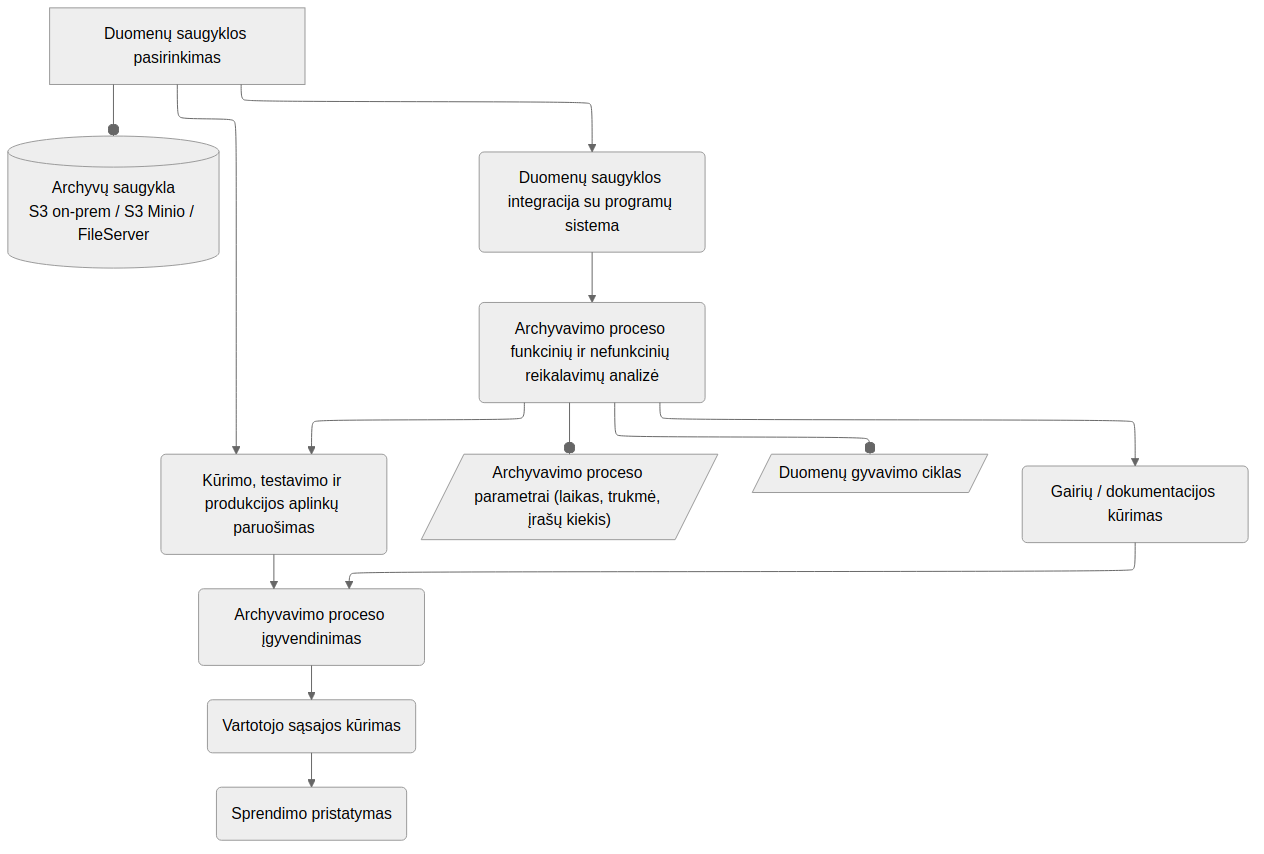
\includegraphics[width=\textwidth]{images/plan.png}
    \caption{Praktinės veiklos planas}
    \label{fig:plan}
\end{figure}

\section{Įmonės apibūdinimas}

\subsection{Įmonės organizacinė struktūra}
\SEB~yra vienas didžiausių Lietuvoje veikiančių komercinių bankų, priklauso Švedijos bankininkystės grupei \textit{Skandinaviska Enskilda Banken} (SEB) ir yra priskiriamas \textit{Baltijos} divizijai. 

\PDT~veikia \textit{Baltijos} divizijoje ir sujungia visų trijų baltijos šalių \textit{SEB} darbuotojus į tarptautines komandas, atsakingas už IT infrastruktūros ir produktų palaikymą ir plėtrą.

\PD~-- \textit{Produktų plėtros ir technologijų centro} departamentas, atsakingas už produktus ir procesus. Čia dirba IT architektai, programų sistemų kūrėjai, testuotojai, verslo analitikai, projektų vadovai ir kiti specialistai. Šio departamento komandos dirba sekdamos \textit{Agile} \cite{cohenIntroductionAgileMethods2004} metodologiją, tad darbo procesai yra dinamiški ir greitai keičiasi reaguojant į pokyčius.

\subsection{Produktų plėtros departamento teikiamos paslaugos}

\PD~nuolat bendradarbiauja su kitais banko departamentais ir klientais, siekdami sukurti ir palaikyti aukštos kokybės produktus. Pagrindinės šio departamento veiklos sritys yra:
\begin{itemize}
    \item \textbf{Produktų plėtra}
    \begin{itemize}
        \item Naujų produktų kūrimas banko klientams ir darbuotojams.
        \item Esamų produktų tobulinimas.
        \item Programų sistemų palaikymas.
    \end{itemize}
    \item \textbf{Procesų optimizavimas} -- esamų procesų tobulinimas ir automatizavimas.
\end{itemize}

\subsection{Sudarytos darbo sąlygos}
Praktikos vietoje galioja atviro ofiso \angl{open office} principas -- nėra atskirų kabinetų, darbuotojai dirba vienoje erdvėje. Tai skatina bendradarbiavimą ir komunikaciją. Kiekvienoje atviroje darbo vietoje yra ergonomiška kėdė, pakeliamas stalas bei du monitoriai.
\section{Praktikos veiklos aprašymas}

\begin{activities}
    \veikla{Duomenų saugyklos pasirinkimas}
    \aprasymas{
        Peržiūrėtos organizacijoje naudojamos duomenų saugyklos. Atrinkti 3 galimi variantai:
        \begin{enumerate}
            \item \textit{S3 on-prem} -- duomenų saugykla, palaikanti S3 protokolą \angl{S3 Compatible Storage}. Ši saugykla veikia organizacijos valdomuose serveriuose, juos prižiūri IT infrastruktūros skyrius.
            % TODO: Add Minio citation
            % milestone: citations
            \item \textit{S3 Minio}~\cite{CITE} -- duomenų saugykla, palaikanti S3 protokolą. Ši saugykla veikia konteinerizuotoje aplinkoje. Kiekviena sistema gali turėti savo \textit{Minio} komponentą ir ten kaupti duomenis. Tokiu atveju už šį komponentą atsakinga sistemą prižiūrinti komanda.
            % TODO: Add SFTO citation
            % milestone: citations
            \item \textit{Failų serveris \angl{File Server}} -- duomenų saugykla, palaikanti SFTP \textit{(Secure File Transfer Protocol)}~\cite{CITE}. Ši saugykla veikia organizacijos valdomuose serveriuose, juos prižiūri IT infrastruktūros skyrius.
        \end{enumerate}

        Dėl organizacijoje priimtos strategijos, failų serverio varianto buvo
        atsisakyta iškart. \textit{S3 Minio} variantas atmestas dėl netinkamo panaudos
        atvejo. Pagal vidinius dokumentus, ši saugykla tinkama aktyviam objektų
        saugojimui ir naudojimui, tačiau neturėtų būti naudojama kaip archyvas. }
    \rezultatai{ Pasirinkta \textit{S3 on-prem} duomenų saugykla. } \row

    \veikla{Kūrimo aplinkos paruošimas}
    \aprasymas{
        \begin{itemize}
            \item Užpildytas \SD~dokumentas infrastruktūros komandai su reikalavimais paruošti
                  kūrimo aplinkai tinkamą \textit{S3 on-prem} duomenų saugyklą. Kūrimo aplinkai
                  numatyti maži saugyklos dydžio reikalavimai bei laisva prieiga prie duomenų
                  saugyklos konfigūracijos.
            \item Dėl organizacijos tinklo architektūros sukurtas tinklo tunelis tarp kūrimo
                  aplinkos ir duomenų saugyklos, leidžiantis kūrimo aplinkai pasiekti duomenų
                  saugyklos tinklo zoną.
        \end{itemize}
    }
    \rezultatai {
        Paruošta saugyklos kūrimo aplinka. Gauti prisijungimo duomenys su administratoriaus teisėmis.
    }
    \row

    \veikla{Duomenų saugyklos integracija su aplikacija}
    \aprasymas{
        Integracija atliekama su \textit{Java} virtualioje mašinoje \angl{Java Virtual Machine -- JVM} veikiančia aplikacija, parašyta naudojant \textit{Spring Boot} karkasą.
        Integracijos žingsniai:
        \begin{enumerate}
            \item S3 SDK \angl{Software Development Kit} bibliotekos konfigūravimas.
            \item S3 komponento, gebančio atlikti pagrindinius veiksmus su duomenų saugykla
                  programavimas. Praktikos užduoties kontekste pagrindiniai veiksmai suprantami
                  kaip:
                  \begin{itemize}
                      \item duomenų įkėlimas į duomenų saugyklą,
                      \item individualių duomenų atsiuntimas iš duomenų saugyklos,
                      \item duomens paieška pagal identifikatorių ar jo pradžią \angl{prefix},
                      \item asinchroninis išlygiagretintas didelio duomenų kiekio įkėlimas į duomenų
                            saugyklą.
                  \end{itemize}
            \item S3 komponento funkcijų jungiklio \angl{feature flag} konfigūravimas.
            \item S3 komponento modulių testavimas.
            \item Rankinis S3 komponento testavimas.
        \end{enumerate}
    }
    \rezultatai {
        Sėkmingai įgyvendinta duomenų saugyklos integracija su aplikacija.
    }
    \row

    \veikla{Archyvavimo proceso funkcinių ir nefunkcinių reikalavimų analizė}
    \aprasymas{
        Funkcinių ir nefunkcinių reikalavimų analizė atlikta kalbantis su programų sistemų kūrėjais, verslo analitikais bei sprendimų architektais. Svarbiausios įžvalgos iš šių vartotojų:
        \begin{itemize}
            \item Kartais reikalinga galimybė atlikti paiešką pagal sudėtingas SQL užklausas,
                  ypač naujesniems versijavimo duomenims.
            \item Verslo analitikai neturi galimybės patys peržiūrėti versijavimo duomenų, tad
                  dažniausiai kreipiasi į programų sistemų kūrėjus.
            \item Su duomenų bazėje esamu duomenų kiekiu pirmasis archyvavimas gali užtrukti
                  kelias dienas, o tai sulėtintų sistemos darbą.
        \end{itemize}
    }
    \rezultatai{
        \textbf{Funkciniai reikalavimai:}
        \begin{itemize}
            \item Archyvavimo procesas turi archyvuoti senesnius, nei 3 mėnesių versijavimo
                  duomenis.
            \item Versijavimo duomenys turi būti pasiekiami per grafinę vartotojo sąsają.
            \item Grafinėje vartotojo sąsajoje turi būti galimybė palyginti 2 tokio pat tipo
                  įrašus.
            \item Archyvavimo procesas turi vykti nakties metu.
        \end{itemize}

        \textbf{Nefunkciniai reikalavimai:}
        \begin{itemize}
            \item Archyvavimo procesas turi užtrukti \le 1h.
            \item (\rightarrow \textit{išvestinis reikalavimas}) Archyvavimo procesas vienu metu turi archyvuoti \le 1M vieno tipo įrašų.
        \end{itemize}
        
        % TODO(!Data): Add Data Lifecycle diagram 
        % 
    }
    \row

\end{activities}
\section{Rezultatai, išvados ir pasiūlymai}

\subsection{Darbo rezultatai ir išvados}

\subsubsection*{Pagrindiniai rezultatai}

\begin{itemize}
    \item Išanalizuotos organizacijoje naudojamos objektų saugojimo technologijos ir pasirinkta tinkamiausia specifiniam panaudos atvejui (specifinių programos duomenų archyvavimui) -- \textit{S3 on-prem}.
    \item Programų sistemai suprogramuotas integracijos su \textit{S3 on-prem} sistema komponentas.
    \item Surinkti bei dokumentuoti archyvavimo proceso reikalavimai.
    \item Programų sistemai suprogramuotas archyvavimo proceso komponentas.
    \item Paruoštas sprendimas įdiegtas visose aplinkose.
\end{itemize}

\subsubsection*{Išvados}

\begin{itemize}
    \item Architektūrinis sprendimas integraciją su \textit{S3 on-prem} įgyvendinti kaip atskirą komponentą yra lankstus tiek panaudos atvejų, tiek duomenų, tiek infrastruktūros požiūriu. Pavyzdžiui, kuriant bei įgyvendinant naujus procesus, generuojančius archyvavimui tinkamus duomenis, galima naudotis jau esamu komponentu ir archyvavimą įtraukti į pradinį proceso įgyvendinimą.
    \item Archyvavimo procesas sprendžia gan paprastą problemą ir iš esmės nėra sudėtingas, tačiau surinkus reikalavimus iš naudotojų, sprendimų architektų, organizacijos vidinių tvarkų bei teisės aktų tampa akivaizdu, jog proceso įgyvendinimas -- netrivialus.
    \item Atlikus sprendimo diegimą visose aplinkose galima teigti, jog pagrindinis praktikos tikslas -- \enquote{sukurti automatizuotą versiavimo įrašų archyvavimo sprendimą} -- įgyvendintas.
    \item Atlikus skaičiavimus su duomenų bazėje esančiu duomenų kiekiu nustatyta, jog po \sim  2 mėn. duomenų bazės versijavimo įrašų lentelė užims \sim 20 kartų mažiau vietos. Tai leidžia teigti, jog pagrindinis praktikos uždavinys -- \enquote{atlaisvinti vietą duomenų bazėje ir sumažinti jos apkrovą} -- pasiektas.
\end{itemize}

\subsection{Praktikos darbo privalumai ir trūkumai}

\subsubsection*{Privalumai}
\begin{itemize}
    \item Praktikos užduotis apėmė visas programų sistemų inžinerijos proceso dalis -- reikalavimų rinkimą, analizę, sprendimo architektūros kūrimą, programavimą, testavimą, diegimą ir dokumentavimą.
    \item Praktikos užduotis buvo atliekama \textit{Agile} komandoje dalyvaujant visose komandos veiklose ir procesuose. Tai atitiko realias darbo sąlygas.
\end{itemize}

\subsubsection*{Trūkumai}

Profesinė praktika atitiko jai keliamus reikalavimus ir lūkesčius, trūkumų nenustatyta.

\subsection{Žinių įvertinimas}
Profesinės praktikos metu įgytos ar pagilintos šios žinios ir įgūdžiai:
\begin{itemize}
    \item Objektų saugojimo \angl{object storage} technologijos, jų panaudos atvejai \angl{use cases}.
    \item S3 sąsaja \angl{S3 API}.
    \item \textit{Spring Boot} karkasas \angl{framework}.
    \item \textit{Web MVC} karkasas.
    \item \textit{Agile} metodologija.
    \item Komandinis darbas.
    \item Automatinis testavimas.
    \item Pakeitimų valdymas.
    \item Programų sistemų konfigūracijos valdymas ir CaC \angl{Configuration as Code}.
\end{itemize}

Praktikos metu, lyginant su universitete gautomis žiniomis, įgyta daugiau specifinių ir konkretesnių žinių, tiesiogiai taikomų praktikoje. Pavyzdžiui, objektų saugimo technologijos nėra dėstomos universitete, tačiau tai tėra specifinio duomenų saugojimo sprendimo abstrakcija, o pagrindinės duomenų saugojimo technologijos -- duomenų bazės -- yra dėstomos universitete.

Panaši situacija yra ir su karkasais -- tai yra specifinės technologijos, apie kurias universitete susipažįstama objektinio programavimo ir programų sistemų kūrimo kursuose.

Apie \textit{Agile} metodologiją, komandinį darbą bei automatinį testavimą yra universiteto paskaitose kalbama plačiai ir išreikštinai, tad praktikoje šios žinios buvo pritaikytos ir įtvirtintos. 

Pakeitimų valdymas ir programų sistemų konfigūracijos valdymas yra itin svarbūs procesai, kuriuose dalyvauja kiekvienas komandos narys, tačiau universitete apie šiuos procesus buvo tik užsiminta. Praktikos metu įsigilinti į šiuos procesus nėra pakankamai laiko, tad įgytos tik pradinės žinios.

\subsection{Rekomendacijos universitetui}

\subsubsection*{DevOps / DevSecOps}

Dažnai už programinės įrangos kūrimą atsakingos komandos taip pat yra dalinai ar visiškai atsakingos ir už programinės įrangos infrastruktūros valdymą. Programų sistemų kūrėjams neretai tenka valdyti programinės įrangos konfigūraciją, tinklo, duomenų bazių prieigą, atlikti telemetriją bei analizuoti programinės įrangos veikimą. Tai yra operacinė \textit{DevOps} dalis. Be to, šių dienų praktikos rodo, jog saugumo užtikrinimas taip pat neretai pereina iš vienos centrinės saugumo komandos organizacijoje į kūrimo ir palaikymo komandas -- \textit{DevSecOps}. Taigi, studentai turėtų būti ne tik supažindinami su šiomis praktikomis, bet ir ruošiami kaip programų sistemų kūrimo, palaikymo, infrastruktūros, operacijų bei saugumo specialistai. 

\subsubsection*{Debesijos technologijos}

Debesijos \angl{cloud} technologijos per pastarąjį dešimtmetį tapo itin populiarios ir dažnai įrašomos IT įmonių strategijose. Debesija ne tik suteikia daug galimybių, bet ir kelia tam tikrus reikalavimus programų sistemų architektūrai, į kuriuos būtina atsižvelgti kuriant praktiškai bet kokią verslui vertę nešančią sistemą. Autoriaus nuomone, universitetas turėtų supažindinti studentus su debesijos technologijomis detaliai aptariant ir pagrindinius privalomus priimti sprendimus kuriant programų sistemas. Taip pat universitetas turėtų suteikti žinias ir galimybę studentams išbandyti debesijos technologijas praktiškai.

\printbibliography[title = {Literatūra ir šaltiniai}]


\end{document}
